\documentclass[12pt,a4paper]{article}
\usepackage[utf8]{inputenc}
\usepackage[spanish]{babel}
\usepackage{graphicx}
\usepackage{float}
\usepackage{geometry}
\usepackage{xcolor}
\usepackage{hyperref}
\usepackage{listings}
\usepackage{caption}
\geometry{top=2.5cm, bottom=2.5cm, left=2.5cm, right=2.5cm}

% Configuración de listings para código Dart (opcional)
\lstdefinelanguage{Dart}{
  keywords={import, class, final, var, void, Future, String, int, bool, dynamic, @override, Widget, State, StatefulWidget, StatelessWidget, Text, Column, Row, Container, Scaffold, AppBar, ListView, Card, ListTile, FloatingActionButton, Icon, IconButton, PopupMenuButton, Dialog, AlertDialog, TextField, Navigator, MaterialPageRoute, Hive, Box, ValueListenableBuilder, Draggable, DragTarget, AnimatedContainer},
  keywordstyle=\color{blue}\bfseries,
  identifierstyle=\color{black},
  commentstyle=\color{gray},
  stringstyle=\color{red},
  sensitive=true,
  morecomment=[l]{//},
  morecomment=[s]{/*}{*/},
  morestring=[b]',
  morestring=[b]"
}
\lstset{
  language=Dart,
  basicstyle=\ttfamily\small,
  numbers=left,
  numberstyle=\tiny,
  stepnumber=1,
  tabsize=2,
  showspaces=false,
  showstringspaces=false,
  breaklines=true,
  frame=single,
  backgroundcolor=\color{white}
}

\title{\textbf{Smart Notes App} \\ \large Proyecto IHC}
\author{Aaron Rodrigo Ramos Reyes \\ Universidad Autónoma Metropolitana - Unidad Cuajimalpa}
\date{\today}

\begin{document}

\maketitle
\thispagestyle{empty}
\newpage

\tableofcontents
\newpage

\section{Introducción}
Smart Notes es una aplicación móvil desarrollada en Flutter que permite gestionar notas personales organizadas en grupos (carpetas). El proyecto implementa funcionalidades de arrastrar y soltar, personalización de colores, historial de edición (Undo/Redo) y persistencia local mediante Hive. Este documento describe la arquitectura, tecnologías empleadas, flujo de uso, funciones implementadas y las áreas de mejora previstas para la próxima entrega.

\section{Tecnologías utilizadas}
\begin{itemize}
    \item \textbf{Lenguaje:} Dart 3.x
    \item \textbf{Framework:} Flutter 3.x
    \item \textbf{Persistencia local:} Hive + Hive Flutter (NoSQL, rápido y nativo)
    \item \textbf{Generación de código:} build\_runner, hive\_generator
    \item \textbf{IDE:} Visual Studio Code
    \item \textbf{Control de versiones:} Git
\end{itemize}

\section{Arquitectura del proyecto}
La aplicación sigue una arquitectura basada en capas simplificada, típica de Flutter:
\begin{itemize}
    \item \textbf{Capa de presentación:} Widgets (screens, diálogos, widgets reutilizables).
    \item \textbf{Capa de lógica de negocio:} Servicios (NoteService, GroupService) y manejo de estado con ValueNotifier + ValueListenableBuilder.
    \item \textbf{Capa de datos:} Modelos (Note, NoteGroup) y adaptadores Hive.
\end{itemize}

\subsection{Diagrama de clases}
\begin{figure}[H]
    \centering
    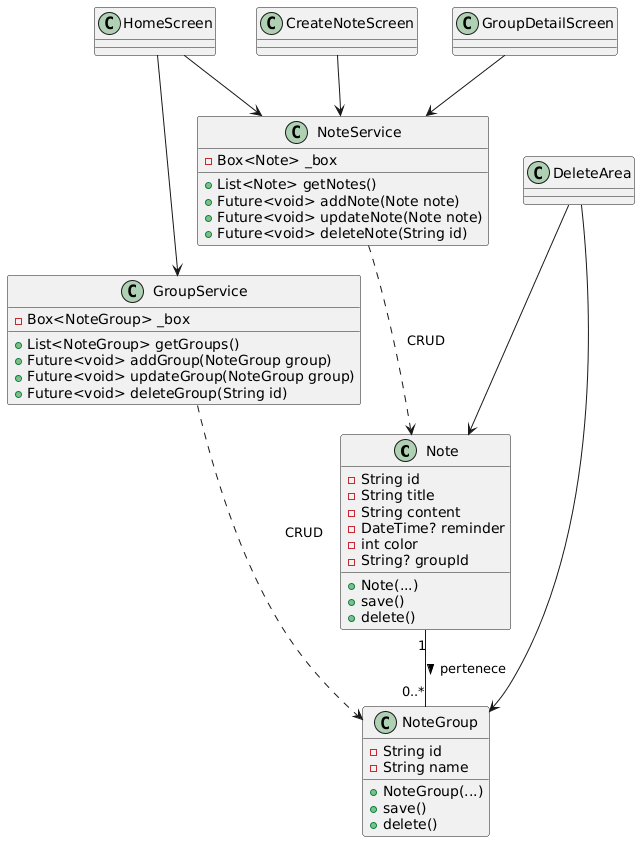
\includegraphics[width=\textwidth]{imagenes/clases.png}
    \caption{Diagrama de clases UML (generado con PlantUML). Muestra las relaciones entre modelos, servicios y widgets principales.}
    \label{fig:clases}
\end{figure}

\subsection{Diagrama de flujo (agregar nota)}
\begin{figure}[H]
    \centering
    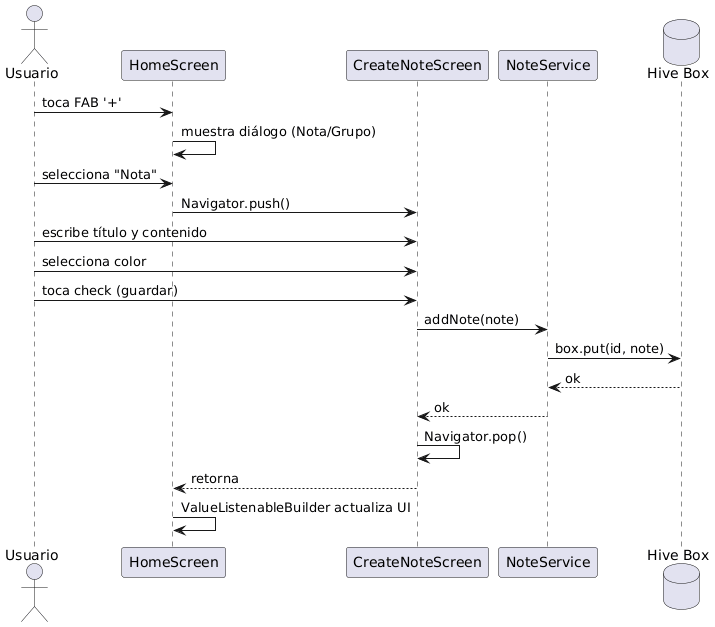
\includegraphics[width=0.8\textwidth]{imagenes/flujo.png}
    \caption{Flujo de creación de una nota desde el botón flotante hasta la persistencia en Hive.}
    \label{fig:flujo}
\end{figure}

\subsection{Código PlantUML}
Para generar los diagramas anteriores, utiliza el siguiente código en \href{https://www.plantuml.com/}{PlantUML}:

\subsubsection*{Diagrama de clases (clases.puml)}
\begin{lstlisting}[basicstyle=\ttfamily\footnotesize]
@startuml
class Note {
  - String id
  - String title
  - String content
  - DateTime? reminder
  - int color
  - String? groupId
  + Note(...)
  + save()
  + delete()
}
class NoteGroup {
  - String id
  - String name
  + NoteGroup(...)
  + save()
  + delete()
}
class NoteService {
  - Box<Note> _box
  + List<Note> getNotes()
  + Future<void> addNote(Note note)
  + Future<void> updateNote(Note note)
  + Future<void> deleteNote(String id)
}
class GroupService {
  - Box<NoteGroup> _box
  + List<NoteGroup> getGroups()
  + Future<void> addGroup(NoteGroup group)
  + Future<void> updateGroup(NoteGroup group)
  + Future<void> deleteGroup(String id)
}
class HomeScreen
class CreateNoteScreen
class GroupDetailScreen
class DeleteArea

Note "1" -- "0..*" NoteGroup : pertenece >
NoteService ..> Note : CRUD
GroupService ..> NoteGroup : CRUD
HomeScreen --> NoteService
HomeScreen --> GroupService
GroupDetailScreen --> NoteService
CreateNoteScreen --> NoteService
DeleteArea --> Note
DeleteArea --> NoteGroup
@enduml
\end{lstlisting}

\subsubsection*{Diagrama de flujo (flujo\_agregar\_nota.puml)}
\begin{lstlisting}[basicstyle=\ttfamily\footnotesize]
@startuml
actor Usuario
participant "HomeScreen" as H
participant "CreateNoteScreen" as C
participant "NoteService" as S
database "Hive Box" as DB

Usuario -> H: toca FAB '+'
H -> H: muestra dialogo (Nota/Grupo)
Usuario -> H: selecciona "Nota"
H -> C: Navigator.push()
Usuario -> C: escribe titulo y contenido
Usuario -> C: selecciona color
Usuario -> C: toca check (guardar)
C -> S: addNote(note)
S -> DB: box.put(id, note)
DB --> S: ok
S --> C: ok
C -> C: Navigator.pop()
C --> H: retorna
H -> H: ValueListenableBuilder actualiza UI
@enduml
\end{lstlisting}

\section{Flujo de uso}
A continuación se describen las interacciones principales del usuario con la aplicación.

\subsection{Captura: Pantalla principal}
\begin{figure}[H]
    \centering
    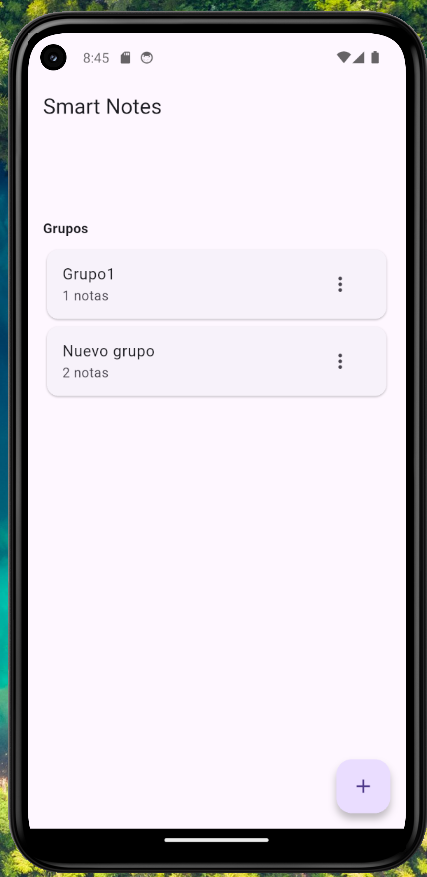
\includegraphics[width=0.4\textwidth]{imagenes/home.png}
    \caption{Pantalla principal (HomeScreen). Muestra listado de notas sin grupo y grupos.}
    \label{fig:home}
\end{figure}

\subsection{Captura: Crear/Editar nota}
\begin{figure}[H]
    \centering
    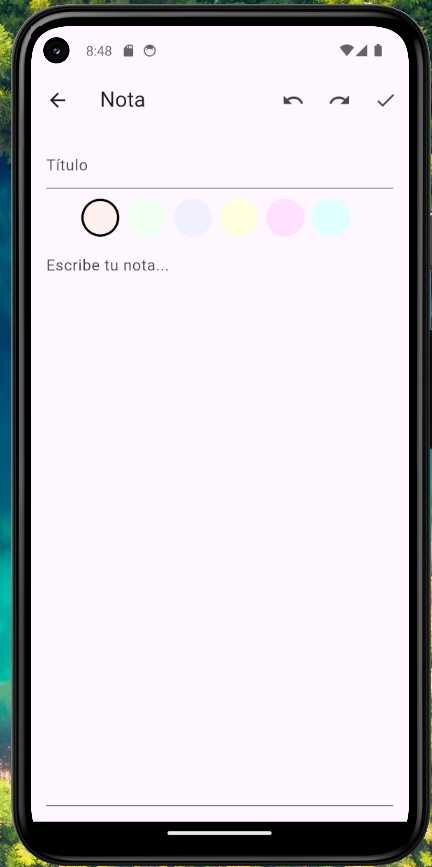
\includegraphics[width=0.4\textwidth]{imagenes/captura_create_note.png}
    \caption{Pantalla de creación/edición de nota. Incluye selector de colores pastel y botones Undo/Redo.}
    \label{fig:create}
\end{figure}

\subsection{Captura: Detalle de grupo}
\begin{figure}[H]
    \centering
    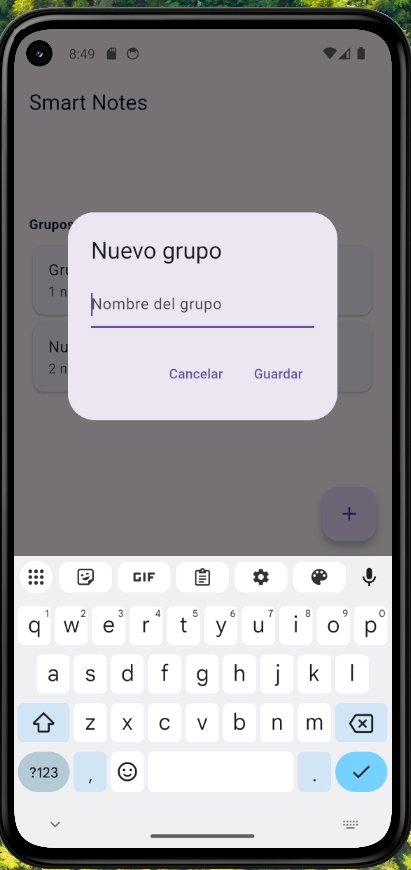
\includegraphics[width=0.4\textwidth]{imagenes/captura_group.png}
    \caption{Pantalla de detalle de grupo. Muestra las notas pertenecientes y menú para editar/eliminar el grupo.}
    \label{fig:group}
\end{figure}

\subsection{Captura: Área de borrado por arrastre}
\begin{figure}[H]
    \centering
    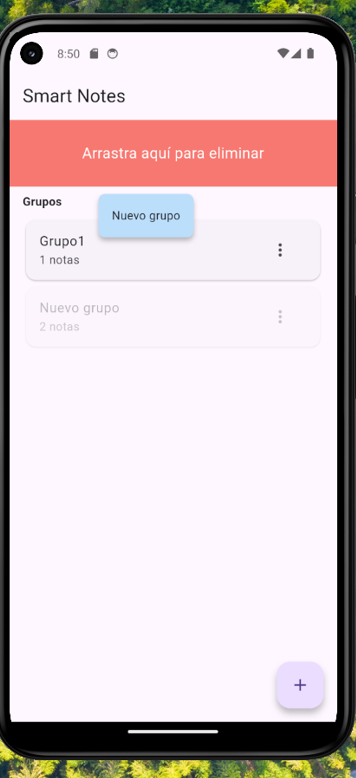
\includegraphics[width=0.4\textwidth]{imagenes/borrado_por_arrastre.png}
    \caption{Área superior que aparece al arrastrar una nota o grupo; soltar allí elimina el elemento previa confirmación.}
    \label{fig:delete}
\end{figure}

\subsection{Captura: Menu nota/carpeta}
\begin{figure}[H]
    \centering
    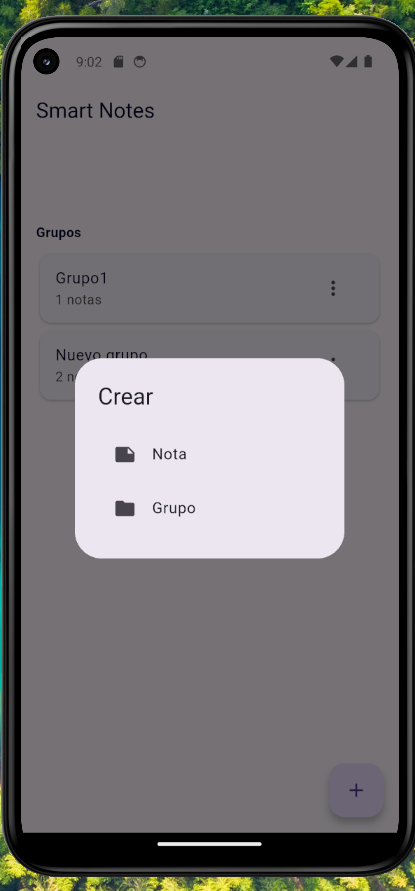
\includegraphics[width=0.4\textwidth]{imagenes/menu_nota_carpeta.png}
    \caption{Menú contextual que permite la creacion de notas o grupos.}
    \label{fig:menu}
\end{figure}

\subsection{Captura: Menu nota}
\begin{figure}[H]
    \centering
    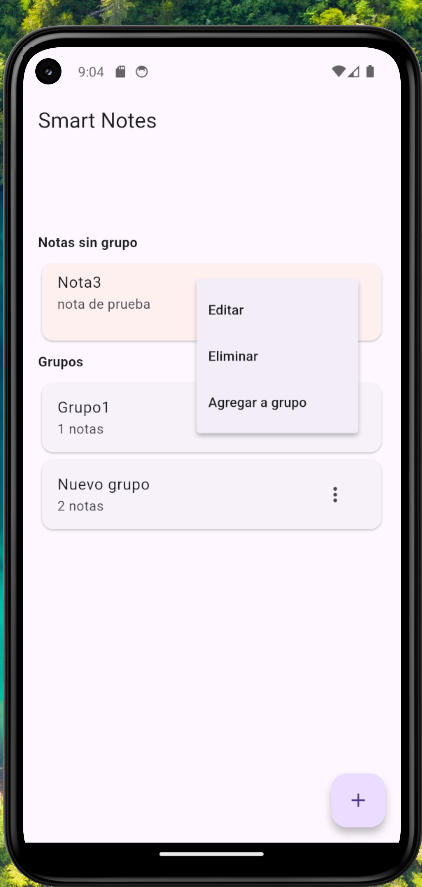
\includegraphics[width=0.4\textwidth]{imagenes/menu_capturas.png}
    \caption{Menú contextual que permite eliminar, editar o agrupar notas.}
    \label{fig:menu_capturas}
\end{figure}
\subsection{Captura: Menu carpeta}
\begin{figure}[H]
    \centering
    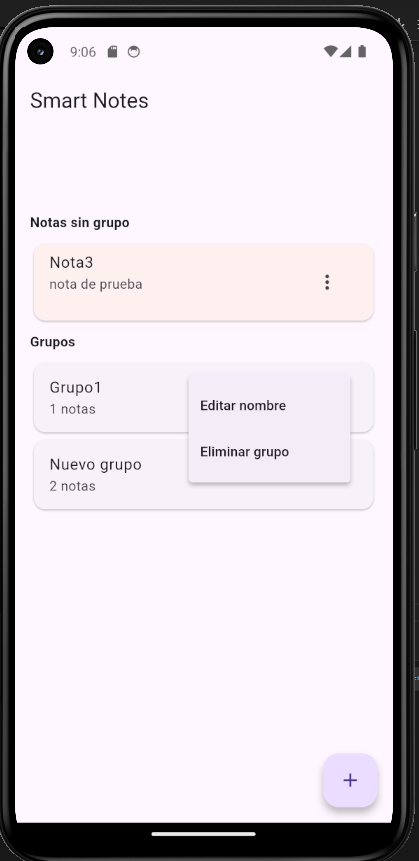
\includegraphics[width=0.4\textwidth]{imagenes/menu_carpeta.png}
    \caption{Menú contextual de una carpeta. Muestra opciones de edición, eliminación}
    \label{fig:menu_carpeta}
\end{figure}


\section{Funciones principales}
\begin{itemize}
    \item \textbf{Creación de notas:} título, contenido, color pastel, recordatorio (opcional).
    \item \textbf{Edición de notas:} modificar cualquier campo, con historial de contenido (Undo/Redo).
    \item \textbf{Eliminación:} mediante botón en menú contextual o arrastrando al área de borrado (siempre con confirmación).
    \item \textbf{Grupos (carpetas):} crear, editar nombre, eliminar (las notas se desasignan automáticamente).
    \item \textbf{Asignación de notas a grupos:} desde el menú de tres puntos en cada nota o arrastrando una nota sobre un grupo.
    \item \textbf{Arrastrar y soltar:}
        \begin{itemize}
            \item Nota sobre otra nota → crea un grupo automático con ambas.
            \item Nota sobre un grupo → asigna la nota a ese grupo.
            \item Nota/grupo al área superior → elimina (confirmación).
        \end{itemize}
    \item \textbf{Personalización:} 6 colores pastel para el fondo de las notas.
    \item \textbf{Persistencia:} todos los datos se guardan localmente con Hive.
\end{itemize}

\section{Áreas a mejorar para la próxima entrega}
Tras una primera ronda de levantamiento de requerimientos, se han identificado las siguientes mejoras y nuevas funcionalidades:

\subsection{Integración de Inteligencia Artificial}
\begin{itemize}
    \item \textbf{Reconocimiento de texto (OCR):} el usuario podrá tomar una foto o seleccionar una imagen de la galería y extraer el texto para convertirlo automáticamente en una nota.
    \item \textbf{Reconocimiento de voz:} dictado de notas mediante micrófono, transcribiendo el audio a texto en tiempo real.
    \item \textbf{Sugerencias inteligentes:} basado en el contenido de la nota, la IA propondrá:
        \begin{itemize}
            \item Creación de una carpeta temática (ej. si la nota habla de “recetas”, sugerirá crear o añadir a una carpeta “Cocina”).
            \item Establecer recordatorios automáticos detectando fechas, horas o frases como “mañana”, “próximo lunes”.
        \end{itemize}
\end{itemize}

\subsection{Comodities y experiencia de usuario}
\begin{itemize}
    \item \textbf{Arrastrar nota a carpeta:} actualmente es posible arrastrar una nota sobre otra y formar un grupo automático sin embargo se busca que al arrastar una nota a un grupo ya establecido se agrege de manera automática.
    \item \textbf{Selector de color global:} al elegir un color para una nota, la pantalla de edición adoptará temporalmente (mientras se encuentre dento de la nota) ese color de fondo para ofrecer una vista previa inmersiva.
    \item \textbf{Selección múltiple:} manteniendo presionada una nota (sin arrastrar) se activará un modo de selección que permita marcar varias notas. Las acciones disponibles serán:
        \begin{itemize}
            \item Eliminar todas las seleccionadas.
            \item Asignar todas a un mismo grupo.
            \item Crear un nuevo grupo con todas las seleccionadas.
        \end{itemize}
    \item \textbf{Otros comodities:} búsqueda global de notas.
\end{itemize}

\section{Conclusiones}
Smart Notes ha logrado implementar un sistema funcional de notas con organización por grupos, interacciones táctiles avanzadas (drag \& drop, menús contextuales) y una interfaz limpia y personalizable. La arquitectura basada en Hive garantiza rapidez y facilidad de mantenimiento. Las mejoras propuestas elevarán la aplicación a un nivel superior, haciéndola más inteligente y cómoda para el usuario final.

\end{document}